\section{Edge colouring and group properties}
\newcommand{\colA}{\colorEdgeA}
\newcommand{\colB}{\colorEdgeB}
\newcommand{\colC}{\colorEdgeC}
\newcommand{\width}{very thick}
\frame{\tableofcontents[currentsection]}


\begin{frame}{Embedding questions}
    \uncover<2->{
        Given: A triangular complex
    }
    \begin{itemize}
        \item<3-> Can it be embedded into $\R^3$?
        \item<4-> In how many ways?
    \end{itemize}
    \uncover<5->{
        Simplifications:
    }
    \begin{enumerate}
        \item<6-> Only simplicial surfaces (that are built from triangles)
        \item<7-> All triangles are isometric
    \end{enumerate}
    \uncover<9->{
        $\leadsto$ Edge--colouring encodes different lengths
    }
    \uncover<8->{
            \begin{center}
                %       F
                %    C     E 
                % A     B    D
                \begin{tikzpicture}[scale=0.9]
                    \coordinate (A) at (0,0);
                    \coordinate (B) at (3,0);
                    \coordinate (C) at (1,1);
                    \coordinate (D) at ($2*(B)$);
                    \coordinate (E) at ($(B)+(C)$);
                    \coordinate (F) at ($2*(C)$);

                    \only<8>{
                        \draw (A) -- (B) -- (D) -- (E) -- (B) -- (C) -- (E) -- (F) -- (C) -- (A);
                    }

                    \uncover<9->{
                        \draw[\colA, \width] (A) -- (B) -- (D);
                        \draw[\colA, \width] (C) -- (E);
                        \draw[\colB, \width] (B) -- (C);
                        \draw[\colB, \width] (D) -- (E) -- (F);
                        \draw[\colC, \width] (A) -- (C) -- (F);
                        \draw[\colC, \width] (B) -- (E);
                    }
                \end{tikzpicture}
            \end{center}
    }
\end{frame}


\begin{frame}{Colouring as permutation}
    \onslide<2->{
        Consider tetrahedron \onslide<3->{with edge colouring}
    }
    \begin{center}
        \begin{tikzpicture}[scale=0.8]
                \coordinate (A) at (0,0);
                \coordinate (B) at (2,0);
                \coordinate (C) at (1,1.4);
                \coordinate (D) at ($2*(B)$);
                \coordinate (E) at ($(B)+(C)$);
                \coordinate (F) at ($2*(C)$);
            \onslide<2->{
                \draw (A) -- (B) -- (D) -- (E) -- (F) -- (C) -- (E) -- (B) -- (C) -- (A);
                \node at (barycentric cs:A=1,B=1,C=1) {1};
                \node at (barycentric cs:B=1,C=1,E=1) {2};
                \node at (barycentric cs:B=1,D=1,E=1) {3};
                \node at (barycentric cs:C=1,E=1,F=1) {4};
                \draw[dotted,thick] ($(A)!0.5!(C)$) to[bend left] ($(C)!0.5!(F)$);
                \draw[dotted,thick] ($(A)!0.5!(B)$) to[bend right] ($(B)!0.5!(D)$);
                \draw[dotted,thick] ($(D)!0.5!(E)$) to[bend right] ($(E)!0.5!(F)$);
            }
            \onslide<3->{
                \draw[\colA, \width] (A) -- (B) -- (D);
                \draw[\colA, \width] (C) -- (E);
                \draw[\colB, \width] (B) -- (C);
                \draw[\colB, \width] (D) -- (E) -- (F);
                \draw[\colC, \width] (A) -- (C) -- (F);
                \draw[\colC, \width] (B) -- (E);
            }

            % Draw switching arrows
            \onslide<7-9>{
                \draw[<->,\colB, thick] (barycentric cs:A=1,B=2,C=2) to[bend left] (barycentric cs:B=2,C=2,E=1);
            }
            \onslide<8-9>{
                \draw[<->,\colB,thick] (barycentric cs:B=1,D=2,E=2) to[bend right=60] (barycentric cs:E=2,F=2,C=1);
            }
            \onslide<10>{
                \draw[<->,\colA,thick] (barycentric cs:A=2,B=2,C=1) to[bend right=60] (barycentric cs:B=2,D=2,E=1);
                \draw[<->,\colA,thick] (barycentric cs:C=2,E=2,B=1) to[bend left] (barycentric cs:C=2,E=2,F=1);
            }
            \onslide<11>{
                \draw[<->,\colC,thick] (barycentric cs:A=2,B=1,C=2) to[bend left=60] (barycentric cs:C=2,E=1,F=2);
                \draw[<->,\colC,thick] (barycentric cs:B=2,C=1,E=2) to[bend left] (barycentric cs:B=2,D=1,E=2);
            }
        \end{tikzpicture}
    \end{center}
    \onslide<4->{
        \textit{simplicial surface} $\Rightarrow$ \onslide<5->{at most two faces at each edge}
    
        \begin{itemize}
            \item<6->[$\leadsto$] every edge defines a transposition of incident faces
            \item<9->[$\leadsto$] every colour class defines a permutation of the faces
            \item<7-> \textcolor{\colB}{(1,2)}\onslide<8->{\textcolor{\colB}{(3,4)}}
                    \onslide<10->{, \textcolor{\colA}{(1,3)(2,4)}}
                    \onslide<11->{, \textcolor{\colC}{(1,4)(2,3)}}
            \item<12->[$\leadsto$] group theoretic considerations
                \begin{itemize}
                    \item<13-> The connected components of the surface correspond to 
                        \onslide<14->{the orbits of $\langle 
                            \textcolor{\colA}{\sigma_a}, 
                            \textcolor{\colB}{\sigma_b}, 
                            \textcolor{\colC}{\sigma_c}\rangle$ on
                        the faces}
                        \onslide<15->{
                            (fast computation for permutation groups)
                        }
                \end{itemize}
        \end{itemize}
    }
\end{frame}
         

\begin{frame}{How do faces fit together?}
    \onslide<2->{
        Consider a face of the surface \onslide<3->{and a neighbouring face.}
    }

    \onslide<4->{
        The neighbour can be coloured in two ways:
    }
    \onslide<1->{
        \begin{center}
        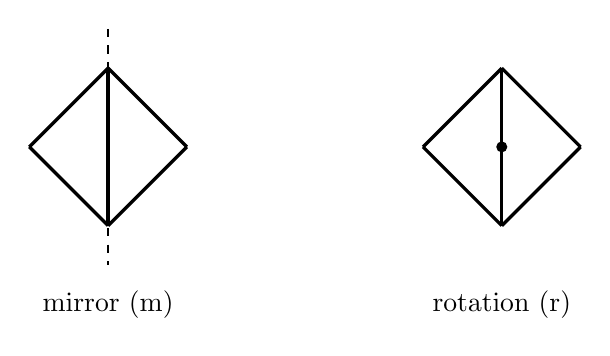
\begin{tikzpicture}
            % Numbers to determine drawing
            \def\x{1}
            \def\y{1}

            %      B
            %    / | \
            %   A  |  D
            %    \ | /
            %      C
            
            % First pair
            \begin{scope}
                \coordinate (A) at (0,0);
                \coordinate (B) at (\x,\y);
                \coordinate (C) at (\x,-\y);
                \coordinate (D) at (2*\x,0);

                \onslide<2->{
                    \draw[\colA,\width] (A) -- (B);
                    \draw[\colB,\width] (A) -- (C);
                    \draw[\colC,\width] (B) -- (C);
                }
                \onslide<3->{
                    \draw (B) -- (D) -- (C);
                }
                \onslide<5->{
                    \draw[\colA,\width] (B) -- (D);
                    \draw[\colB,\width] (C) -- (D);
                }
                \onslide<7->{
                    % Draw mirror line
                    \draw[dashed, thick] (\x,1.5*\y) -- (\x,-1.5*\y);
                    \node at (\x,-2*\y) {mirror (m)};
                }
            \end{scope}

            % Second pair
            \begin{scope}[xshift=5cm]
                \coordinate (A) at (0,0);
                \coordinate (B) at (\x,\y);
                \coordinate (C) at (\x,-\y);
                \coordinate (D) at (2*\x,0);

                \onslide<4->{
                    \draw[\colA,\width] (A) -- (B);
                    \draw[\colB,\width] (A) -- (C);
                    \draw[\colC,\width] (B) -- (C);
                    \draw (B) -- (D) -- (C);
                }
                \onslide<6->{
                    \draw[\colB,\width] (B) -- (D);
                    \draw[\colA,\width] (C) -- (D);
                }
                \onslide<8->{
                    % Draw rotation center and circle
                    \fill[black] (\x,0) circle (2pt);
                    \node[scale=2] at (\x,0) {$\circlearrowleft$};
                    \node at (\x,-2*\y) {rotation (r)};
                }
            \end{scope}
        \end{tikzpicture}
        \end{center}
    }
    \onslide<9->{
        This gives an \textbf{mr--assignment} for the edges of the surface.
    }

    \onslide<10->{
        \begin{lem}
            Permutations and mr--assignment uniquely determine the surface.
        \end{lem}
    }
\end{frame}


\begin{frame}{Constructing surfaces from groups}
    \pause
    A general mr--assignment leads to complicated surfaces.
    
    \pause
    Simplification: edges of same colour have the same mr--type

    \pause
    Example
        \begin{center}
            \begin{tikzpicture}
                \coordinate (A) at (0,0);
                \coordinate (B) at (2,0);
                \coordinate (C) at (1,1.4);
                \coordinate (D) at ($2*(B)$);
                \coordinate (E) at ($(B)+(C)$);
                \coordinate (F) at ($2*(C)$);

                \draw (A) -- (B) -- (D) -- (E) -- (F) -- (C) -- (E) -- (B) -- (C) -- (A);
                \node at (barycentric cs:A=1,B=1,C=1) {1};
                \node at (barycentric cs:B=1,C=1,E=1) {2};
                \node at (barycentric cs:B=1,D=1,E=1) {3};
                \node at (barycentric cs:C=1,E=1,F=1) {4};
                
                \draw[dotted,thick] ($(A)!0.5!(C)$) to[bend left] ($(C)!0.5!(F)$);
                \draw[dotted,thick] ($(A)!0.5!(B)$) to[bend right] ($(B)!0.5!(D)$);
                \draw[dotted,thick] ($(D)!0.5!(E)$) to[bend right] ($(E)!0.5!(F)$);

                \draw[\colA, \width] (A) -- (B) -- (D);
                \draw[\colA, \width] (C) -- (E);
                \draw[\colB, \width] (B) -- (C);
                \draw[\colB, \width] (D) -- (E) -- (F);
                \draw[\colC, \width] (A) -- (C) -- (F);
                \draw[\colC, \width] (B) -- (E);
            \end{tikzpicture}
        \end{center}
    \pause
    has only r--edges.
\end{frame}


\begin{frame}{The mirror--case}
    \pause
    If all edges are mirrors, the situation is simple.
    \pause
    \begin{lem}
        A simplicial surface has only mirror--edges iff it covers a 
        single triangle\pause, i.\,e. there is a surjective incidence--preserving
        map \pause to the simplicial surface consisting of exactly one face.
    \end{lem}
    \pause
    Consider
        \begin{center}
            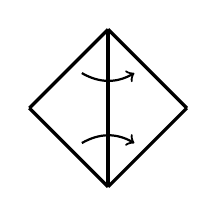
\begin{tikzpicture}
                \def\x{1}
                \def\y{1}

                \coordinate (A) at (0,0);
                \coordinate (B) at (\x,\y);
                \coordinate (C) at (\x,-\y);
                \coordinate (D) at (2*\x,0);

                    \draw[\colA,\width] (A) -- (B);
                    \draw[\colB,\width] (A) -- (C);
                    \draw[\colC,\width] (B) -- (C);
                    \draw (B) -- (D) -- (C);
                    \draw[\colA,\width] (B) -- (D);
                    \draw[\colB,\width] (C) -- (D);

                \def\mid{3}
                \def\near{5}
                \draw[->,thick] (barycentric cs:A=\mid,B=\near,C=1) to[bend right] (barycentric cs:B=\near,C=1,D=\mid);
                \draw[->,thick] (barycentric cs:A=\mid,B=1,C=\near) to[bend left] (barycentric cs:B=1,C=\near,D=\mid);
            \end{tikzpicture}
        \end{center}
    \begin{itemize}
        \pause
        \item[$\Rightarrow$] Unique map that preserves incidence
        \pause
        \item Covering pulls back a mirror--colouring of the triangle.
        \pause
        \item Mirror--colouring defines a map to the triangle.
    \end{itemize}
\end{frame}


\begin{frame}[fragile]{Construction from permutations}
    \onslide<2->{
        Start with three involutions 
        \textcolor{\colA}{$\sigma_a$}, 
        \textcolor{\colB}{$\sigma_b$}, \textcolor{\colC}{$\sigma_c$} 
        in permutation representation
        \onslide<3->{(like generators of a finite group)}
    }

    \onslide<4->{
    \begin{lem}
        There exists a coloured surface with the given involutions
        \onslide<5->{where all edges are mirror edges.}
    \end{lem}
    }

    \begin{itemize}
        \item<6-> The faces are the points moved by the involution triple
        \item<7-> The edges are the 1- and 2--cycles of the involutions
        \item<8-> The vertices are \onslide<11->{the orbits of 
            $\langle \textcolor{\colA}{\sigma_a}, 
            \textcolor{\colB}{\sigma_b} \rangle$
            on the faces} \onslide<12->{(for all pairs)}
    \end{itemize}

    \onslide<9->{
    \begin{center}
    \begin{tikzpicture}
        %     P2 ---- P1 ---- Q3
        %    /  \    /  \   /  \
        %   /    \  /    \ /    \
        % P3 ---- Z ---- P0 ---- Q2
        %   \    /  \    /  \   /
        %    \  /    \  /    \ /
        %     P4 ---- P5 ---- Q1

        % Define the coordinates
        \def\rad{1.5}
        \coordinate (Z) at (0,0);
        \foreach \i in {0,1,2,3,4,5}
            \coordinate (P\i) at (60*\i:\rad);

        \foreach \i in {1,2,3}
            \coordinate (Q\i) at ($(P0) + (-120+60*\i:\rad)$);
        
        % Draw the circle around Z
        \foreach \i/\j in {0/1, 1/2, 2/3, 3/4, 4/5, 5/0}{
            \draw[\colC, \width] (P\i) -- (P\j);
        }

        % Draw the spokes of Z
        \foreach \i in {0,2,4}
            \draw[\colA,\width] (Z) -- (P\i);

        \foreach \i in {1,3,5}
            \draw[\colB,\width] (Z) -- (P\i);

        % Draw missing lines around P0
        \draw[\colB, \width] (P5) -- (Q1) -- (Q2) -- (Q3) -- (P1);
        \draw[\colA, \width] (Q1) -- (P0) -- (Q3);
        \draw[\colC, \width] (P0) -- (Q2);

        % Draw the continuations
        \foreach \p/\q/\z in {P1/P2/Z, P2/P3/Z, P3/P4/Z, P4/P5/Z, P5/Q1/P0, Q1/Q2/P0, Q2/Q3/P0, Q3/P1/P0}
            \draw[gray!50!black, dotted, thick] ($(\p)!0.5!(\q)$) -- (barycentric cs:\z=-0.5,\p=1,\q=1);

        % Draw the vertices
        \foreach \p in {Z,P0}
            \fill[gray] (\p) circle (2pt);

        % Draw the arc segments (center, outer, first, second, colour)
        \newcommand{\arcSeg}[5]{
            \draw[#5, thick, <->] (barycentric cs:#1=4,#2=2,#3=1) to[bend right] (barycentric cs:#1=4,#2=2,#4=1);
        }
        \onslide<10->{
        \arcSeg{Z}{P1}{P0}{P2}{\colB}
        \arcSeg{Z}{P2}{P1}{P3}{\colA}
        \arcSeg{Z}{P3}{P2}{P4}{\colB}
        \arcSeg{Z}{P4}{P3}{P5}{\colA}
        \arcSeg{Z}{P5}{P4}{P0}{\colB}
        \arcSeg{Z}{P0}{P5}{P1}{\colA}
        }

        \onslide<12->{
        \arcSeg{P0}{Q3}{Q2}{P1}{\colA}
        \arcSeg{P0}{P1}{Q3}{Z}{\colC}
        \arcSeg{P0}{Z}{P1}{P5}{\colA}
        \arcSeg{P0}{P5}{Z}{Q1}{\colC}
        \arcSeg{P0}{Q1}{P5}{Q2}{\colA}
        \arcSeg{P0}{Q2}{Q1}{Q3}{\colC}
        }
    \end{tikzpicture}
    \end{center}
    }
\end{frame}


\begin{frame}[fragile]{Construction example}
    \onslide<2->{ $\textcolor{\colA}{\sigma_a} = \textcolor{\colA}{(1,2)(3,4)(5,6)(7,8)}$\\ }
    \onslide<3->{ $\textcolor{\colB}{\sigma_b} = \textcolor{\colB}{(1,4)(2,3)(5,8)(6,7)}$\\ }
    \onslide<4->{ $\textcolor{\colC}{\sigma_c} = \textcolor{\colC}{(1,5)(2,6)(3,7)(4,8)}$\\ }

    \begin{center}
    \begin{tikzpicture}
        % Coordinates
        \coordinate (Z) at (0,0);
        \foreach \i in {0,1,2,3,4}
            \coordinate (P\i) at (60*\i:2);
        \foreach \i/\j in {0/1, 1/2, 2/3, 3/4}
            \coordinate (Q\i\j) at ($(P\i)+(P\j)$);

        \newcommand{\vertex}[1]{
            \fill[black] (#1) circle (3pt);
        }
        \newcommand<>{\vertArc}[3]{
            \def\dist{0.2}
            \onslide#4{
                \filldraw[draw=black, fill=black!50!white] (#1) -- 
                    ($(#1)!\dist!(#2)$) to[bend right=25] ($(#1)!\dist!(#3)$) -- cycle;
            }
        }

        % Draw the arcs first (since faces have to be drawn on top)
        
        % 1
        \vertArc<6-10>{Z}{P1}{P2}
        \vertArc<11-13>{P2}{Z}{P1}
        \vertArc<16>{P1}{P2}{Z}
        
        % 2
        \vertArc<7-10>{Z}{P2}{P3}
        \vertArc<11-13>{P2}{P3}{Z}
        \vertArc<14-15>{P3}{Z}{P2}

        % 3
        \vertArc<8-10>{Z}{P3}{P4}
        \vertArc<14-15>{P3}{P4}{Z}
        \vertArc<18>{P4}{Z}{P3}

        % 4
        \vertArc<9-10>{Z}{P0}{P1}
        \vertArc<16>{P1}{Z}{P0}
        \vertArc<18>{P0}{P1}{Z}

        % 5
        \vertArc<12-13>{P2}{P1}{Q12}
        \vertArc<16>{P1}{Q12}{P2}
        \vertArc<19>{Q12}{P2}{P1}

        % 6
        \vertArc<13>{P2}{Q23}{P3}
        \vertArc<14-15>{P3}{P2}{Q23}
        \vertArc<19>{Q23}{P3}{P2}

        % 7
        \vertArc<15>{P3}{Q34}{P4}
        \vertArc<18>{P4}{P3}{Q34}
        \vertArc<19>{Q34}{P4}{P3}

        % 8
        \vertArc<16>{P1}{P0}{Q01}
        \vertArc<18>{P0}{Q01}{P1}
        \vertArc<19>{Q01}{P1}{P0}


        % First vertex

        % 1
        \onslide<5->{
            \node at (barycentric cs:Z=1,P1=1,P2=1) {1};
            \draw[\colA,\width] (Z) -- (P2);
            \draw[\colB,\width] (Z) -- (P1);
            \draw[\colC,\width] (P1) -- (P2);
        }

        % 2
        \onslide<7->{
            \node at (barycentric cs:Z=1,P2=1,P3=1) {2};
            \draw[\colB,\width] (Z) -- (P3);
            \draw[\colC,\width] (P2) -- (P3);
        }

        % 3
        \onslide<8->{
            \node at (barycentric cs:Z=1,P3=1,P4=1) {3};
            \draw[\colC,\width] (P3) -- (P4);
            \draw[\colA,\width] (Z) -- (P4);
        }

        % 4
        \onslide<9->{
            \node at (barycentric cs:Z=1,P0=1,P1=1) {4};
            \draw[\colA,\width] (Z) -- (P0);
            \draw[\colC,\width] (P0) -- (P1);
        }

        \onslide<10->{
            \draw[\colA,\width,dotted] ($(Z)!0.5!(P4)$) to[bend right] ($(Z)!0.5!(P0)$);
        }

        \onslide<6-10>{
            \vertex{Z}
        }


        % Second vertex

        % 5
        \onslide<12->{
            \node at (barycentric cs:P1=1,P2=1,Q12=1) {5};
            \draw[\colB,\width] (P1) -- (Q12);
            \draw[\colA,\width] (P2) -- (Q12);
        }

        % 6
        \onslide<13->{
            \node at (barycentric cs:P2=1,P3=1,Q23=1) {6};
            \draw[\colA,\width] (P2) -- (Q23);
            \draw[\colA,\width,dotted] ($(P2)!0.5!(Q23)$) to[bend left] ($(P2)!0.5!(Q12)$);
            \draw[\colB,\width] (P3) -- (Q23);
        }

        \onslide<11-13>{
            \vertex{P2}
        }


        % Third vertex

        % 7
        \onslide<15->{
            \node at (barycentric cs:P3=1,P4=1,Q34=1) {7};
            \draw[\colB,\width] (P3) -- (Q34);
            \draw[\colB,\width,dotted] ($(P3)!0.5!(Q23)$) to[bend right] ($(P3)!0.5!(Q34)$);
            \draw[\colA,\width] (P4) -- (Q34);
        }

        \onslide<14-15>{
            \vertex{P3}
        }

        % Fourth vertex

        % 8
        \onslide<16->{
            \node at (barycentric cs:P0=1,P1=1,Q01=1) {8};
            \draw[\colB,\width] (P1) -- (Q01);
            \draw[\colB,\width,dotted] ($(P1)!0.5!(Q01)$) to[bend right] ($(P1)!0.5!(Q12)$);
            \draw[\colA,\width] (P0) -- (Q01);
        }
        \onslide<16>{
            \vertex{P1}
        }


        \onslide<17->{
            \draw[\colA,\width,dotted] ($(P0)!0.5!(Q01)$) to[bend left=60] ($(P4)!0.5!(Q34)$);
        }

        % Fifth vertex
        \onslide<18>{
            \vertex{P0}
            \vertex{P4}
        }

        % Sixth vertex
        \onslide<19>{
            \vertex{Q01}
            \vertex{Q12}
            \vertex{Q23}
            \vertex{Q34}
        }


        \begin{scope}[xshift=6cm]
            % Coordinates of octahedron
                \def\len{2} % The length of the base
                \def\h{1}   % \h*\len is the hight of the apex above the 
                            % center of the square
                \coordinate (Mid) at (0,0);
                \coordinate (Right) at (0.5*\len,0.3*\len);
                \coordinate (Left) at (-0.75*\len,0.25*\len);
                \coordinate (Back) at ($(Right)+(Left)$);
                \coordinate (Center) at ($(Left)!0.5!(Right)$);
                \coordinate (Up) at ($(Center)+(0,\h*\len)$);
                \coordinate (Down) at ($(Center)+(0,-\h*\len)$);

                \onslide<20->{
                    \draw[\colA,\width] (Up) -- (Mid) -- (Down);
                    \draw[\colA,\width,dashed] (Up) -- (Back) -- (Down);
                    \draw[\colB,\width] (Up) -- (Right) -- (Down) -- (Left) -- cycle;
                    \draw[\colC,\width] (Left) -- (Mid) -- (Right);
                    \draw[\colC,\width,dashed] (Left) -- (Back) -- (Right);

                    %\node at (barycentric cs:Mid=1,Down=1,Right=1) {1};
                    %\node at (barycentric cs:Mid=1,Down=1,Left=1) {2};
                    %\node at (barycentric cs:Mid=1,Up=1,Right=1) {5};
                    %\node at (barycentric cs:Mid=1,Up=1,Left=1) {6};
                    
                    % Vertices to hide drawing problems in edge meetings
                    \foreach \p in {Mid,Right,Left,Back,Up,Down}
                        \fill[gray] (\p) circle (1pt);
                }
        \end{scope}
    \end{tikzpicture}
    \end{center}
\end{frame}


\begin{frame}[fragile]{Net of an icosahedron}
    \uncover<2->{
        \textcolor{blue}{gap$>$ }\textcolor{red}{\texttt{DrawSurfaceToTikZ$($iko,"NetIko.tex"$)$;}}
    }
    \begin{itemize}
        \item<4-> Has to be manually untangled
    \end{itemize}
    
    \uncover<3->{
        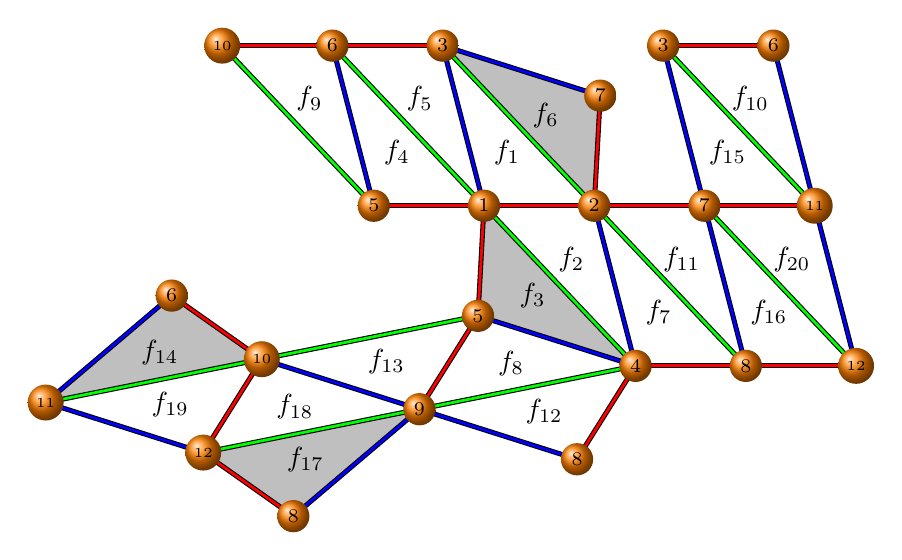
\begin{tikzpicture}[scale=0.7]
            \coordinate (V1_1) at (0, 0);
            \coordinate (V2_1) at (2, 0);
            \coordinate (V3_1) at (-0.75, 2.904737509655563);
            \coordinate (V3_2) at (3.25, 2.904737509655563);
            \coordinate (V4_1) at (2.75, -2.904737509655563);
            \coordinate (V5_1) at (-0.109375, -1.997007037888199);
            \coordinate (V5_2) at (-2, 3.33066907387547e-16);
            \coordinate (V6_1) at (-2.75, 2.904737509655563);
            \coordinate (V6_2) at (5.25, 2.904737509655562);
            \coordinate (V6_3) at (-5.6650390625, -1.630132638882223);
            \coordinate (V7_1) at (2.109375, 1.997007037888199);
            \coordinate (V7_2) at (4, -3.33066907387547e-16);
            \coordinate (V8_1) at (4.75, -2.904737509655563);
            \coordinate (V8_2) at (1.6875, -4.599167723621307);
            \coordinate (V8_3) at (-3.4599609375, -5.631711135256683);
            \coordinate (V9_1) at (-1.171875, -3.691437251853944);
            \coordinate (V10_1) at (-4.75, 2.904737509655564);
            \coordinate (V10_2) at (-4.03125, -2.783706780086581);
            \coordinate (V11_1) at (6, -6.661338147750939e-16);
            \coordinate (V11_2) at (-7.953125000000001, -3.570406522284963);
            \coordinate (V12_1) at (6.75, -2.904737509655564);
            \coordinate (V12_2) at (-5.09375, -4.478136994052326);
            
            
            \fill[white] (V1_1) -- (V2_1) -- (V3_1) -- cycle;
            \node (F1) at (0.4166666666666666, 0.9682458365518543) {$f_{1}$};
            \fill[white] (V1_1) -- (V2_1) -- (V4_1) -- cycle;
            \node (F2) at (1.583333333333333, -0.9682458365518543) {$f_{2}$};
            \fill[lightgray] (V1_1) -- (V4_1) -- (V5_1) -- cycle;
            \node (F3) at (0.8802083333333333, -1.633914849181254) {$f_{3}$};
            \fill[white] (V1_1) -- (V5_2) -- (V6_1) -- cycle;
            \node (F4) at (-1.583333333333333, 0.9682458365518546) {$f_{4}$};
            \fill[white] (V1_1) -- (V3_1) -- (V6_1) -- cycle;
            \node (F5) at (-1.166666666666667, 1.936491673103709) {$f_{5}$};
            \fill[lightgray] (V2_1) -- (V3_1) -- (V7_1) -- cycle;
            \node (F6) at (1.119791666666667, 1.633914849181254) {$f_{6}$};
            \fill[white] (V2_1) -- (V4_1) -- (V8_1) -- cycle;
            \node (F7) at (3.166666666666667, -1.936491673103709) {$f_{7}$};
            \fill[white] (V4_1) -- (V5_1) -- (V9_1) -- cycle;
            \node (F8) at (0.4895833333333333, -2.864393933132569) {$f_{8}$};
            \fill[white] (V5_2) -- (V6_1) -- (V10_1) -- cycle;
            \node (F9) at (-3.166666666666667, 1.936491673103709) {$f_{9}$};
            \fill[white] (V3_2) -- (V6_2) -- (V11_1) -- cycle;
            \node (F10) at (4.833333333333333, 1.936491673103708) {$f_{10}$};
            \fill[white] (V2_1) -- (V7_2) -- (V8_1) -- cycle;
            \node (F11) at (3.583333333333333, -0.9682458365518546) {$f_{11}$};
            \fill[white] (V4_1) -- (V8_2) -- (V9_1) -- cycle;
            \node (F12) at (1.088541666666667, -3.731780828376938) {$f_{12}$};
            \fill[white] (V5_1) -- (V9_1) -- (V10_2) -- cycle;
            \node (F13) at (-1.770833333333333, -2.824050356609574) {$f_{13}$};
            \fill[lightgray] (V6_3) -- (V10_2) -- (V11_2) -- cycle;
            \node (F14) at (-5.883138020833333, -2.661415313751255) {$f_{14}$};
            \fill[white] (V3_2) -- (V7_2) -- (V11_1) -- cycle;
            \node (F15) at (4.416666666666666, 0.9682458365518537) {$f_{15}$};
            \fill[white] (V7_2) -- (V8_1) -- (V12_1) -- cycle;
            \node (F16) at (5.166666666666666, -1.936491673103709) {$f_{16}$};
            \fill[lightgray] (V8_3) -- (V9_1) -- (V12_2) -- cycle;
            \node (F17) at (-3.241861979166667, -4.600428460387651) {$f_{17}$};
            \fill[white] (V9_1) -- (V10_2) -- (V12_2) -- cycle;
            \node (F18) at (-3.432291666666667, -3.65109367533095) {$f_{18}$};
            \fill[white] (V10_2) -- (V11_2) -- (V12_2) -- cycle;
            \node (F19) at (-5.692708333333333, -3.610750098807956) {$f_{19}$};
            \fill[white] (V7_2) -- (V11_1) -- (V12_1) -- cycle;
            \node (F20) at (5.583333333333333, -0.9682458365518549) {$f_{20}$};
            
            
            \tikzset{EdgeStyle/.style = {thin, double distance=1pt} }
            
            \draw[ EdgeStyle, double=red] (V2_1) -- (V1_1);
            \draw[ EdgeStyle, double=blue] (V1_1) -- (V3_1);
            \draw[ EdgeStyle, double=green] (V4_1) -- (V1_1);
            \draw[ EdgeStyle, double=red] (V5_1) -- (V1_1);
            \draw[ EdgeStyle, double=red] (V1_1) -- (V5_2);
            \draw[ EdgeStyle, double=green] (V1_1) -- (V6_1);
            \draw[ EdgeStyle, double=green] (V3_1) -- (V2_1);
            \draw[ EdgeStyle, double=blue] (V2_1) -- (V4_1);
            \draw[ EdgeStyle, double=red] (V7_1) -- (V2_1);
            \draw[ EdgeStyle, double=red] (V2_1) -- (V7_2);
            \draw[ EdgeStyle, double=green] (V2_1) -- (V8_1);
            \draw[ EdgeStyle, double=red] (V6_1) -- (V3_1);
            \draw[ EdgeStyle, double=red] (V3_2) -- (V6_2);
            \draw[ EdgeStyle, double=blue] (V3_1) -- (V7_1);
            \draw[ EdgeStyle, double=blue] (V7_2) -- (V3_2);
            \draw[ EdgeStyle, double=green] (V3_2) -- (V11_1);
            \draw[ EdgeStyle, double=blue] (V4_1) -- (V5_1);
            \draw[ EdgeStyle, double=red] (V8_1) -- (V4_1);
            \draw[ EdgeStyle, double=red] (V4_1) -- (V8_2);
            \draw[ EdgeStyle, double=green] (V4_1) -- (V9_1);
            \draw[ EdgeStyle, double=blue] (V5_2) -- (V6_1);
            \draw[ EdgeStyle, double=red] (V9_1) -- (V5_1);
            \draw[ EdgeStyle, double=green] (V5_2) -- (V10_1);
            \draw[ EdgeStyle, double=green] (V10_2) -- (V5_1);
            \draw[ EdgeStyle, double=red] (V10_1) -- (V6_1);
            \draw[ EdgeStyle, double=red] (V6_3) -- (V10_2);
            \draw[ EdgeStyle, double=blue] (V6_2) -- (V11_1);
            \draw[ EdgeStyle, double=blue] (V11_2) -- (V6_3);
            \draw[ EdgeStyle, double=blue] (V7_2) -- (V8_1);
            \draw[ EdgeStyle, double=red] (V7_2) -- (V11_1);
            \draw[ EdgeStyle, double=green] (V7_2) -- (V12_1);
            \draw[ EdgeStyle, double=blue] (V8_2) -- (V9_1);
            \draw[ EdgeStyle, double=blue] (V9_1) -- (V8_3);
            \draw[ EdgeStyle, double=red] (V12_1) -- (V8_1);
            \draw[ EdgeStyle, double=red] (V8_3) -- (V12_2);
            \draw[ EdgeStyle, double=blue] (V9_1) -- (V10_2);
            \draw[ EdgeStyle, double=green] (V9_1) -- (V12_2);
            \draw[ EdgeStyle, double=green] (V11_2) -- (V10_2);
            \draw[ EdgeStyle, double=red] (V12_2) -- (V10_2);
            \draw[ EdgeStyle, double=blue] (V11_1) -- (V12_1);
            \draw[ EdgeStyle, double=blue] (V12_2) -- (V11_2);
            
            
            
            \tikzset{VertexStyle/.style = {
             shape = circle,
             ball color = orange,
             text = black,
             inner sep = 2pt,
             outer sep = 0pt,
             minimum size = 8pt} }
            
            \node[VertexStyle] at (V1_1) {\scriptsize 1};
            \node[VertexStyle] at (V2_1) {\scriptsize 2};
            \node[VertexStyle] at (V3_1) {\scriptsize 3};
            \node[VertexStyle] at (V3_2) {\scriptsize 3};
            \node[VertexStyle] at (V4_1) {\scriptsize 4};
            \node[VertexStyle] at (V5_1) {\scriptsize 5};
            \node[VertexStyle] at (V5_2) {\scriptsize 5};
            \node[VertexStyle] at (V6_1) {\scriptsize 6};
            \node[VertexStyle] at (V6_2) {\scriptsize 6};
            \node[VertexStyle] at (V6_3) {\scriptsize 6};
            \node[VertexStyle] at (V7_1) {\scriptsize 7};
            \node[VertexStyle] at (V7_2) {\scriptsize 7};
            \node[VertexStyle] at (V8_1) {\scriptsize 8};
            \node[VertexStyle] at (V8_2) {\scriptsize 8};
            \node[VertexStyle] at (V8_3) {\scriptsize 8};
            \node[VertexStyle] at (V9_1) {\scriptsize 9};
            \node[VertexStyle] at (V10_1) {\tiny 10};
            \node[VertexStyle] at (V10_2) {\tiny 10};
            \node[VertexStyle] at (V11_1) {\tiny 11};
            \node[VertexStyle] at (V11_2) {\tiny 11};
            \node[VertexStyle] at (V12_1) {\tiny 12};
            \node[VertexStyle] at (V12_2) {\tiny 12};

        \end{tikzpicture}
    }
\end{frame}
            

\begin{frame}{Progress report of edge colouring}
    \pause
    Implemented:
    \begin{itemize}
        \pause
        \item computing all colourings of a given simplicial surface
        \pause
        \item constructing all surfaces with given involutions
            \begin{enumerate}
                \pause
                \item up to (coloured) isomorphism
                \pause
                \item with given mr--assignment
            \end{enumerate}
        \pause
        \item drawing of simplicial surfaces
        \pause
        \item constructing various coloured coverings
    \end{itemize}

    \pause
    Still missing:
    \begin{itemize}
        \pause
        \item for which lengths are the surfaces embeddable?
        \pause
        \item can we predict self--intersections?
        \pause
        \item does varying the lengths lead to another embedding?
    \end{itemize}
\end{frame}
